\section{the experiment}
This works focuses on comparing the different miss use models to a reference
calculation in which a single large cascade is build and designed to directly
produce \gls{HEU} from natural uranium.
This works uses the Cyclus fuel cycle simulator to allow material exchange
between facilities.

\subsection{The cascade configuration}
\subsubsection{reference}
As mentioned previously, all the further calculations will be compared to the
most favorable configuration to produce \gls{HEU}, where all the available
centrifuges are used in a single large cascade designed to directly produce \gls{HEU}
from natural uranium, with a tail assay close to $0.3w\%$ uranium. The design
characteristic of the reference cascade are summarized in Table
\ref{tab:cascade_config}.

\subsubsection{default cascade}
The default cascade is the cascade design for normal civilian enrichment
operation, enriching natural uranium to about $3.5w\%$. This cascade will be
layered and fed with uranium at higher enrichment to evaluate the possibility
to used them, with few or no tuning, to produce \gls{HEU}. The characteristics of
the default cascade are summarized in Table \ref{tab:cascade_config}.

\begin{table}[htb]
\centering
  \caption{Summary of cascade design.}
\begin{tabular}{cccc}
\toprule

Cascade Design &       & Reference  & Default    \\
\midrule
Targeted  & Feed       & $0.71w\%$  & $0.71w\%$  \\
Assays    & Product    & $90w\%$    & $4.0w\%$   \\
          & Tail       & $0.3w\%$   & $0.3w\%$   \\
\midrule
Effective & Product    & $90.35w\%$ & $4.13w\%$  \\
Assays    & Tail       & $0.28w\%$  & $0.28w\%$  \\ 
\midrule
Stages    & Enriching  & 4          & 4          \\
Number    & Stripping  & 39         & 10         \\
\bottomrule
\end{tabular}
  \label{tab:cascade_config}
\end{table}


\subsection{scenarios}
Seven different scenarios have been simulated:
\begin{itemize}
\item one as the reference calculation, with a single centrifuges designed to
    produce directly \gls{HEU} from natural uranium,
\item three calculations (one per miss-use model) were default cascade are
    chained to produce \gls{HEU}, without recycling the tails of each cascade,
    the cascade tails are directly sent to the waste,
\item three calculations (one per miss-use model) were default cascade are
    chained to produce \gls{HEU}, the tails of each cascade are recycled, blending
    the tail of one level in the feed of the previous level of
    cascades (see Figure \ref{fig:cascade_level}.
\end{itemize}
In the following, cascades can be connected in tandem, where each set of cascade
in parallel is called a ``level``, as illustrated on Figure
\ref{fig:cascade_level}.

\begin{figure}[ht] % replace 't' with 'b' to force it to be on the bottom
    \centering
    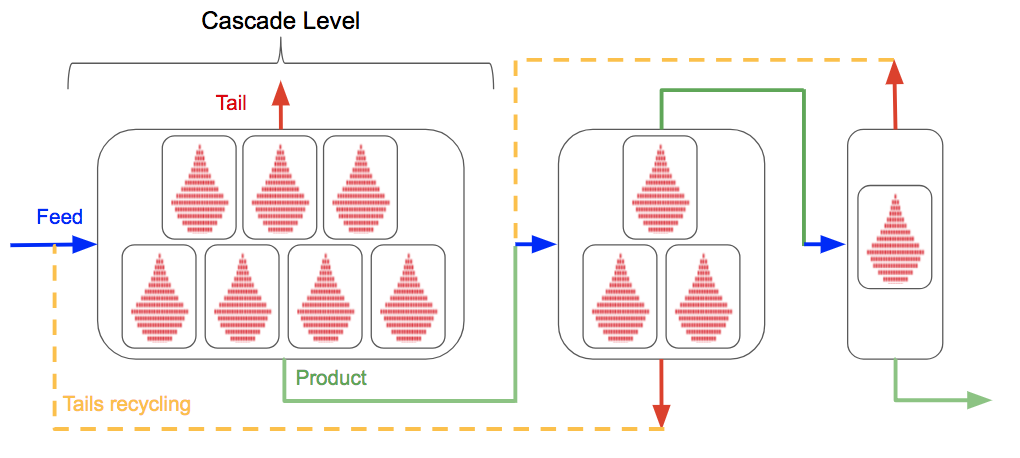
\includegraphics[scale=0.45]{flow}
    \caption{Schematic representation of the chained cascade on three level,
    with the feed, product and the tail flows, respectively in blue, green and
    red. The dashed orange line represent the alternative tail flow with
    recycling them.}
    \label{fig:cascade_level}
\end{figure}


\subsection{Level population}
In order to assign the optimum number of cascade to each level a virtual cut as
been computed as:
\begin{equation}
    \theta^{v}_{i} = \frac{F_{i}-T_{i}}{P_{i}-T_{i}},
\end{equation}
where, i represents a level of cascade and $F_{i}$, $P_{i}$ and $T_{i}$
respectively the feed, product and tail assay of the cascades at this level.

A flow equation similar to \eqref{eq:flow} is then solve to get the optimum
number of cascade per level. When the tail recycling is not enable the
$(1-\theta)$ terms are removed from the flow equation.
The results of the level population are summarized in Table \ref{tab:level}.


\begin{table}[htb]
\centering
  \caption{Summary of cascades level population.}
\begin{tabular}{ccccccccc}
\toprule

Model       &        &           & A         & A         & B         & B       & C         & C          \\
Recycling   &        &           & No        & yes       & No        & Yes     & No        & yes        \\
\midrule                                                                                                 
        &            & Feed      & $0.71w\%$ & $1.3w\%$  & $0.71w\%$ & $0.94w\%$ & $0.71w\%$ & $1.66w\%$ \\
Level 0 & Assay      & Product   & $4.13w\%$ & $7.7w\%$  & $4.13w\%$ & $5.43w\%$ & $4.13w\%$ & $9.53w\%$ \\
        &            & Tail      & $0.29w\%$ & $0.5w\%$  & $0.29w\%$ & $0.39w\%$ & $0.29w\%$ & $0.69w\%$  \\
        & Cascades   &           & 26.73     & 26.45     & 26.6      & 25.8      & 26.73     & 26.45      \\
\midrule                                                                                                 
        &            & Feed      & $4.13w\%$ & $11.9w\%$ & $4.13w\%$ & $6.84w\%$ & $4.13w\%$ & $13.0w\%$ \\
Level 1 & Assay      & Product   & $22.8w\%$ & $55.7w\%$ & $20.6w\%$ & $30.7w\%$ & $20.6w\%$ & $69.8w\%$ \\
        &            & Tail      & $1.8w\%$  & $6.6w\%$  & $1.72w\%$ & $2.91w\%$ & $1.72w\%$ & $9.43w\%$  \\
        & Cascades   &           & 2.92       & 3.20      & 2.91      & 3.41     & 2.92      & 3.20       \\
\midrule                                                                                                 
        &            & Feed      & $22.8w\%$ & $55.7w\%$ & $20.6w\%$ & $34.3w\%$ & $20.6w\%$ & $72.6w\%$ \\
Level 2 & Assay      & Product   & $78.5w\%$ & $95.0w\%$ & $61.0w\%$ & $75.8w\%$ & $61.0w\%$ & $98.4w\%$ \\
        &            & Tail      & $4.12w\%$ & $50.9w\%$ & $9.56w\%$ & $17.5w\%$ & $9.56w\%$ & $69.4w\%$ \\
        & Cascades   &           & 0.31      & 0.35      & 0.37      & 0.64      & 0.31      & 0.35      \\
\midrule                                                                                                 
        &            & Feed      & $78.5w\%$ & N.A.      & $61.0w\%$ & $75.8w\%$ & $61.0w\%$ & N.A.      \\
Level 3 & Assay      & Product   & $98.2w\%$ & N.A.      & $90.4w\%$ & $95.0w\%$ & $90.4w\%$ & N.A.      \\
        &            & Tail      & $76.1w\%$ & N.A.      & $79.3w\%$ & $56.1w\%$ & $38.9w\%$ & N.A.      \\
        & Cascades   &           & 0.03      & N.A.      & 0.080     & 0.18      & 0.03      & N.A.      \\
\bottomrule
\end{tabular}
  \label{tab:cascade_config}
\end{table}

